\subsection{Экономическое взаимодействие}
Великобритания являлась вторым инвестором в экономику России, после Франции. Её особенно интересовали Российская металлургия, нефтяная промышленность.

{\centering \includegraphics[width=\textwidth]{images/Общие\_объёмы-инвестиций.png}}

{\centering 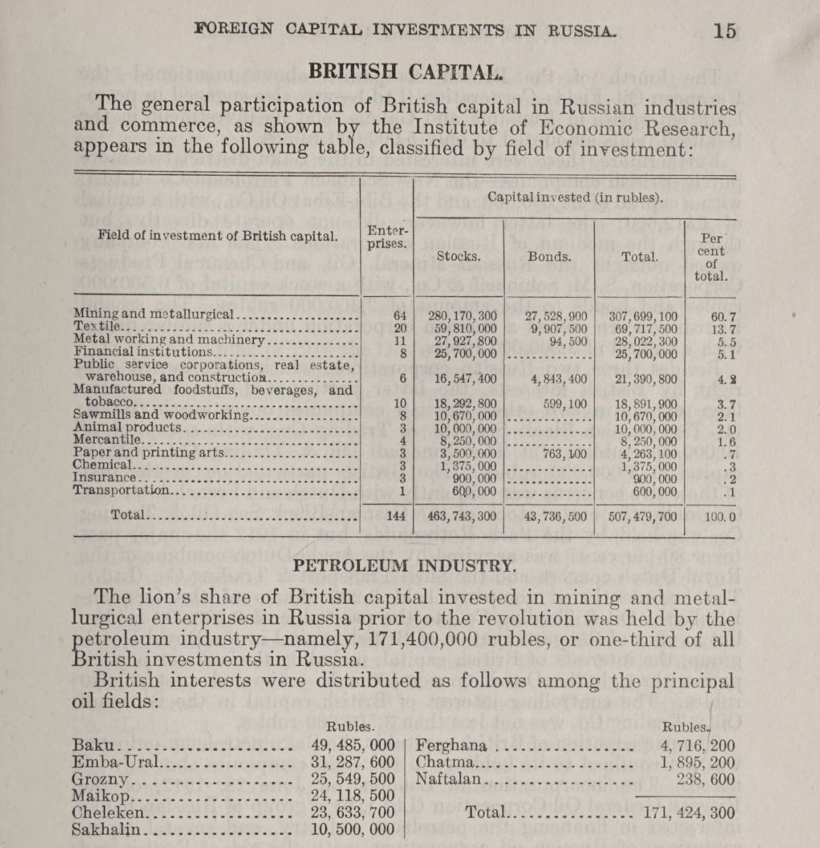
\includegraphics[width=\textwidth]{images/куда-шли-инвестиции.png}}

Данные взяты из Foreign Capital Investments in Russian Industries and Commerce Leonard John Lewery U.S. Government Printing Office